% Generated with TikZ

\documentclass[tikz,border=8pt]{standalone}
\usepackage{tikz}
\usetikzlibrary{calc,positioning,fit,backgrounds}
\usepackage{amsmath}

\tikzset{
  every picture/.append style={
    execute at end picture={
      \begin{scope}[on background layer]
        \draw[rounded corners=6pt, line width=0.8pt, gray!60]
          ([xshift=-6pt,yshift=-6pt]current bounding box.south west) rectangle
          ([xshift=6pt,yshift=6pt]current bounding box.north east);
      \end{scope}
    }
  }
}

\begin{document}
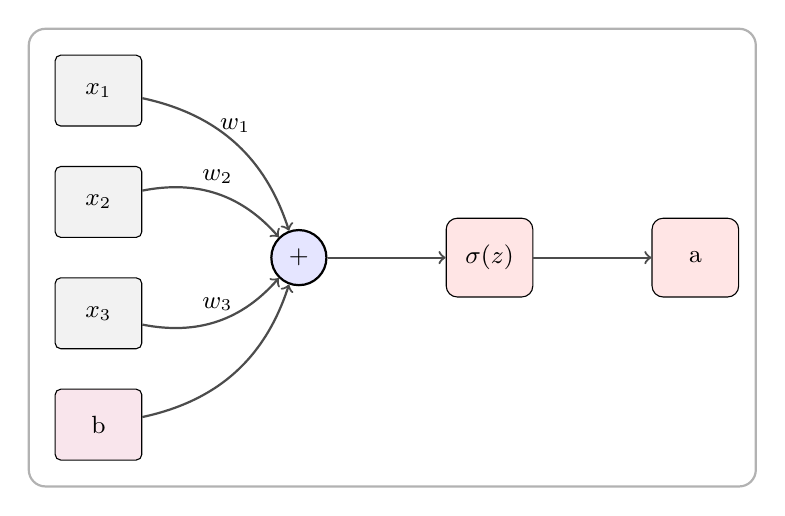
\begin{tikzpicture}[
        node distance=1.4cm,
        font=\small,
        input/.style={draw, rounded corners=2pt, minimum width=1.1cm, minimum height=0.9cm, fill=gray!10},
        bias/.style={draw, rounded corners=2pt, minimum width=1.1cm, minimum height=0.9cm, fill=purple!10},
        oplus/.style={circle, draw, line width=0.8pt, minimum size=0.7cm, fill=blue!10},
        activation/.style={draw, rounded corners=4pt, minimum width=1.1cm, minimum height=1cm, fill=red!10},
        output/.style={draw, rounded corners=4pt, minimum width=1.1cm, minimum height=1cm, fill=red!10},
        arrow/.style={->, thick, draw=black!70},
    ]

    % Input
    \matrix[column sep=0.5cm, row sep=0.5cm] (inputs) {
        \node[input] (x1) {$x_1$};                 \\
        \node[input] (x2) {$x_2$};                 \\
        \node[input] (x3) {$x_3$};                 \\
        \node[bias] (b) {$\mathrm{b}$}; \\
    };
    \node[oplus, right=1.5cm of inputs] (oplus) {$+$};
    \node[activation, right=1.5cm of oplus] (activation) {$\sigma(z)$};
    \node[output, right=1.5cm of activation] (output) {$\mathrm{a}$};

    % Connect bias to oplus
    \draw[arrow, bend left] (x1) to node[midway, above] {$w_1$} (oplus);
    \draw[arrow, bend left] (x2) to node[midway, above] {$w_2$} (oplus);
    \draw[arrow, bend right] (x3) to node[midway, above] {$w_3$} (oplus);
    \draw[arrow, bend right] (b) to (oplus);
    \draw[arrow] (oplus) -- (activation);
    \draw[arrow] (activation) -- (output);

    % Lines

\end{tikzpicture}
\end{document}
